\chapter{Methods}
\label{chap:methods}
This chapter describes the methods used to carry on the research, from the data collection to the preprocessing and the results of the analysis. It includes a brief description of the population that took part into the experiment, the experimental task and conditions, the procedure adopted, and the equipment used. Then it delves into the analysis process starting with the preparation and preprocessing of the data and concluding with the intermediate outcomes of the classification. As previouslyu mentioned, the experiment is the result of a collaboration between the University of Twente, that provided the space, the recruitment system and part of the recording equipment, and myBrainTechnologies that provided their EEG-capable Melomind headsets and the rest of the equipment. The experimental design was reviewed and adjusted for ethical approval by the Ethics Committee of the university with reference number RP 2021-43 and compliant with the safety measures to prevent the spread of the Covid-19 virus.

\section{Experiment}
\label{sec:experiment}
The experimental phase of the research was crucial for the proper evaluation of Melomind. Previous studies conducted internally at myBrainTechnologies provided the theoretical backbone to work with neuromarkers and music, however the datasets of the employees were collected with a different experimental setup that did not account for the continuous measurement of emotional valence and arousal, and in any case there was always a chance data could be biased by the previous knowledge these "expert" subjects had on the topic and the technology. A feasible alternative could have been the simulation of a wearable device, similarly to the approach taken by Wu et al. \cite{wu_estimation_2017}, but that was kept as emergency solution in case it was not possible to run an experiment under the safety restrictions enforced by the Covid-19 pandemic. However, the open datasets available online for emotion analysis \cite{koelstra_deap_2012,soleymani_multimodal_2012,soleymani_deam_nodate} are recorded with a very different equipment than the Melomind, that would have not properly reflected the challenges of using a wearable neural interface. Finally, the opportunity to conduct the study with the students of the University of Twente and the availability of myBrainTechnologies to ship all the technical and hygienic materials to the Netherlands made it possible to proceed with the experimental protocol in the desired conditions.

\subsection{Experimental Annotation app for data collection}
\label{sec:experimental_annotation_app}
An app was developed to collect continuous annotations of perceived emotion, inspired by the design of the FEELTRACE tool \cite{cowie_feeltrace_2000} and the app developed by Thammasan et al. \cite{thammasan_continuous_2016}. The \ac{EA} app was developed in Python using the Psychopy\footnote{https://www.psychopy.org/}  engine for experimental behavioral sciences. The app is a collection of timed routines that alternate guided instructions, annotation tasks on a simplified GUI representing the valence-arousal space and Likert scales to report familiarity/liking scores in the range [1-5]. Three training sessions have been included:
\begin{itemize}
\item T1: the participant is presented with some background information about the \ac{VA} model and how to use the annotation tool.
\item T2: the participant is asked to annotate on the \ac{VA} space the perceived emotion while listening to 2 minutes of mixed music genres.
\item T3: the participant is presented with the simulation of a trial of the experiment, including reporting of familiarity/liking and the two listening conditions (see Chapter \ref{sec:task}).
\end{itemize}

The \ac{EA} app was designed and developed at myBrainTechnologies and then tested with the other employees during a short pilot period to adjust the instructions, the clarity of the GUI and the input method. Two input methods were evaluated with A/B testing methodology, using mouse and joystick respectively. The results of the test (see Appendix \ref{sec:appendix_A1}) confirmed that using mouse as input source required less training and effort, thus softening the cognitive load of the annotation task while music listening. Using the joystick would have enabled collecting annotation even in an eyes-closed listening condition thanks to the tactile feedback, but at the cost of requiring more training and concentration. To record experimental timed events, the \ac{EA} app was connected to the Melomind through a TriggerBox with an USB cable, a customized Arduino Nano board that can send binary-encoded labels using the serial port. 

\subsection{Participants}
\label{sec:participants}
In respect with the Covid-19 safety measures enforced by University of Twente, 45 healthy participants (28 females) participated in the experiment, all students, or ex-students of the university. The mean age of the population is 23.8 ± 3.1, with the oldest student being 31 years old and the youngest student being 18 years old at the time of the experiment (see Appendix \ref{sec:appendix_A2.1}). The lowest educational level was the enrollment as bachelor student and the highest educational level was having completed a master’s degree. Almost half of the participants (20) were Dutch, while all the rest came from different countries, but all of them had at least a C1 or equivalent English proficiency as requirement to enroll in University of Twente. Prior to be confirmed as participants, they were invited through an invitation form informing them on the nature of the experiment and collecting personal information such as demographic information, health conditions, drugs consumption, musical literacy, and some behavioral information on their habits in listening and searching for music to later support the design of a prototype. Almost 5\% of the participants reported to be left-handed, but none asked for an inverted setup of the equipment after it was offered to them (see Appendix \ref{sec:appendix_A2.1}). The only strict criterion to participate in the experiment was the capability to hear music, eventually through a hearing support system. None of the applicants was discarded nor required additional support for their health conditions. Prior to their experimental session, they were asked to refrain from consuming recreational drugs and alcohol in the 12 hours before the experiment and caffeine and tobacco in the hour before the experiment to prevent unexpected biases in the cerebral activity.

\subsection{Stimuli selection}
\label{sec:stimuli}
The stimuli were selected to represent an even as possible distribution of emotions according to the 4 classes identifiable by the quadrants of the Valence-Arousal space. These 4 classes are the possible combinations of positive and negative valence with high and low arousal. To keep consistency with related studies \cite{koelstra_deap_2012}, the classes have been named as follows going clockwise from the top-right quadrant:
\begin{itemize}
\item HAHV: High-Arousal and High-Valence.
\item LAHV: Low-Arousal and High-Valence.
\item LALV: Low-Arousal and Low-Valence.
\item HALV: High-Arousal and Low-Valence.
\end{itemize}
Selecting the right stimuli is a non-trivial task especially in the case of music since many factors can bias the personal perception. For example, familiarity with a certain song might elicit stronger emotions or create an effect of anticipation \cite{sangnark_revealing_2021}, \cite{ward_same_2013}, \cite{salimpoor_anatomically_2011}, while cultural biases or genre preference might completely change how a song is perceived \cite{chang_personalized_2017,fang_perception_2017}. Choosing to include lyrics or no lyrics may shift the attention of the listener from the meaning to the melody and vice versa. It is clearly hard to address all the possible issues but considering the scope of this study and the research on a realistic use-case scenario, most of these factors were either mitigated or considered with the due precautions. 

\begin{figure}[h!]
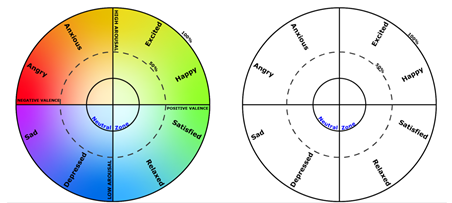
\includegraphics[width=12cm]{img/methods/va_space_experiment.png}
\centering
\caption{The Valence-Arousal space GUI used for the training with color cues on the left, and the uncolored Valence-Arousal space GUI used for the experiment session on the right.} \label{fig_va_space_experiment}
\end{figure}

The stimuli were finally selected as a subset of 8 songs (see Appendix \ref{sec:appendix_A2.2}) from the music database created by Koelstra et al. \cite{koelstra_deap_2012}, according to their emotional tagging. They used the popular online music database last.fm\footnote{https://www.last.fm/}  to retrieve 120 songs with associated music videos through their APIs, emotionally labelled by thousands of users. They then screened them down 40 stimuli during a web assessment session with at least 14 volunteers for each stimulus. The 8 songs selected for this study are a randomly picked subset of those 40 stimuli whose emotional web assessment belonged to the same Valence-Arousal quadrant as the last.fm tagging. For each quadrant there are exactly 2 songs and in total 8 emotions are supposedly portrayed: excitement, happiness, satisfaction, relaxation, depression, sadness, anger, and anxiety. 
It is important to point out that the web assessment conducted by Koelstra et al. was done using the music videos of these songs, and that the placement of the emotions in the \ac{VA} space used in this experiment (see Figure \ref{fig_va_space_experiment}) is a functional simplification of Russel's model \cite{russell_circumplex_1980}.

\subsection{Conditions}
\label{sec:conditions}
There is no common agreement in the academic world on which should be the best recording condition for an \ac{EEG} experiment about emotions, but most researchers agree on the minimization of external stimuli. Only few studies tried to assess the impact of recording in \ac{EO} condition and \ac{EC} condition on emotion analysis. Barry et al. reported \cite{barry_eeg_2007} differences in topography and power levels, due to the processing of visual input, and recommend considering them when choosing baseline conditions. Chang et al. \cite{chang_experiencing_2015} analyzed recording conditions in relation to music listening and reported that frontal Theta power significantly increased in the EC condition, while asymmetries indices in the Alpha power on parietal and temporal sites reflected emotional valence for \ac{EC} and \ac{EO} states respectively. In addition, participants rated music as more pleasant and more positive while listening with their eyes closed. These differences in the listening conditions did not seem to significantly impact on the current study that only used frontal electrodes but were considered in the design of the experimental task and in the choice of the resting state baseline. Another problem is caused by ocular movements and blinks that generates large artifacts in the EEG signal \cite{hagemann_effects_2001}. As a consequence, the data collected is of lower quality and requires more computationally expensive preprocessing. In the worst cases, some data must be pruned or reconstructed, varying from a few channels to the entire dataset of a participant. Eye artifacts are typically found in the data recorded by the electrodes placed on the frontal area of the scalp and are usually filtered away by subtracting \ac{EOG}, if recorded, from the \ac{EEG} signal. However it is not the case of this study that could not take advantage of extra sensors to record \ac{EOG} . In general, we can assume that an \ac{EC} condition yields better quality data than an \ac{EO} condition because the quantity of ocular artifacts will be reduced to the minimum and there is no underlying visual stimuli processing. The downsides of experimenting in the \ac{EC} condition are the obvious limitations on the task that could be presented to the participants and a possible increase of power in the Alpha band of the spectrum, that is usually amplified during resting and focused states. The main advantage of the \ac{EO} condition is the possibility to ask the participants for more complex tasks, at the cost of generating more ocular and muscular artifacts and eventually introducing multiple cognitive tasks at once, that can affect the analysis. Prior to the experiment, we run an internal pilot test at myBrainTechnologies to explore the best compromise options between having good quality data, the maximum amount of data and collecting the behavioral data we needed.
Thammasan et al. \cite{thammasan_continuous_2016} opted for a double listening protocol, in \ac{EC} condition to record \ac{EEG} and in \ac{EO} condition to collect affective annotations. This translates into listening twice to the same song but recording only in the \ac{EC} closed condition and then overlapping the annotations taken during the \ac{EO} conditions. Our limitation of 2 frontal electrodes already constrained the collectable amount of data, so we decided to extend this protocol with a double listening and recording approach, in both conditions. During the pilot we explored the feasibility of collecting annotations in both conditions using a joystick, but then opted for collecting annotations only during \ac{EO} condition with a mouse and then reuse the same annotations on the \ac{EEG} data collected in \ac{EC} condition.  As final consideration, the two conditions can be both present in realistic scenarios, with \ac{EO} being the most common listening condition, for example in an office or free-time scenario in which a user listen to music while performing other cognitive tasks (work, homework, gaming…). Listening in \ac{EC} condition resembles a more relaxed scenario, for example when listening to music at the opera or on a comfortable couch in the evening.

\subsection{Task}
\label{sec:task}
During the experimental session, participants were presented a main task during which their physiological signal were recorded. The task is divided into 3 sub-tasks for both conditions during each trial, with a total of 8 trials. The average length of the recording was approximately 35 minutes of recording. The sub-tasks in each trial, repeated for both conditions, were the following:

\begin{itemize}
\item Listening to white noise: before presenting the stimulus, participants listened to 15 seconds of white noise to “reset” their emotional state.
\item Listening to the stimulus in EO/EC conditions: participants listened to 60 seconds excerpts of each song. During the \ac{EO} condition participants were requested to continuously annotate their emotions on the \ac{VA} space, during the \ac{EC} condition they focused solely on the music. The order of presentation of the conditions depended on the assigned group.
\item Rating the stimulus: after listening to the song, participants were requested to give a rating in terms of familiarity and liking of the excerpts, using Likert scales ranging from 1 to 5. If for any reason they failed to give a score before the 20 seconds timer expired, the score would be automatically set to 3, that represented a neutral answer.
\end{itemize}
So, during each trial, the participants would listen to two different songs, rate them and only annotate during the \ac{EO} condition (see Fig. \ref{fig_experimental_trial}). 

\begin{figure}[h!]
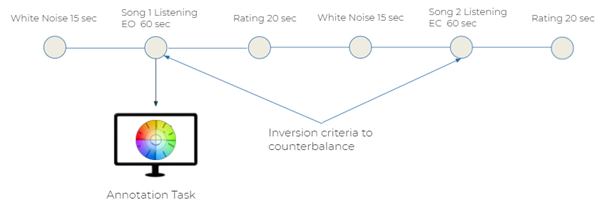
\includegraphics[width=12cm]{img/methods/experimental_trial.png}
\centering
\caption{Diagram of an experimental trial starting with EO listening condition.} \label{fig_experimental_trial}
\end{figure}

It is important to underline that the order of the conditions might induce some bias in the annotation task and the rating of each stimulus. To minimize the statistical effects, participants were randomly assigned to two groups in equal distribution, ECEO and EOEC, according to an inversion criterion that would determine the order in which the conditions were presented during the entire session. This solution seemed more elegant and less confusing than fully randomizing the order of the conditions for each trial, possibly creating confusion in the instructions. In addition, instead to presenting the same song consecutively in both conditions, we decided to split the session into two parts in which the stimuli are presented in pseudo-random class order in the first part, and then inverted in the second part as shown in Figure \ref{fig_inversion_criterion}.

\begin{figure}[h!]
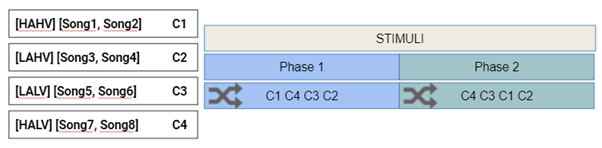
\includegraphics[width=12cm]{img/methods/inversion_criterion.png}
\centering
\caption{Pseudo randomization scheme. Participants listen to all songs twice, in both conditions, during the two parts of the experiment.} \label{fig_inversion_criterion}
\end{figure}

This approach also reduces the familiarity effect caused by listening twice to the same song in a short span of time and mitigates cases of extreme emotional fluctuation within each trial, for example if a very sad song would be followed by a very happy song and then again another sad song. This emotional fluctuation phenomenon cannot be fully eliminated, but it is statistically balanced by the pseudo-randomization of the order in which the classes are presented. 

\subsection{Equipment}
\label{sec:equipment}
During the pilot test some technical issues with the Melomind Q+ forced the use of the standard Melomind (Fig. \ref{fig_melomind}) in frontal setup using electrodes placed over [AF3 AF4] positions of the 10-20 system, thus reducing the amount of recording electrodes from 4 to 2 and requiring to adapt accordingly the entire research. The Melomind was connected via USB cable to a laptop through a TriggerBox and via Bluetooth to a smartphone to remotely control the start and end of the acquisition with  the proprietary Acquisier app developed by myBrainTechnologies. An Empatica E4  wristband was used to collect bio signals from the non-dominant wrist of the participant, namely: \ac{BVP}, body temperature, \ac{HR} and \ac{EDA} (Fig. \ref{fig_empatica}). 

\begin{figure}[h!]
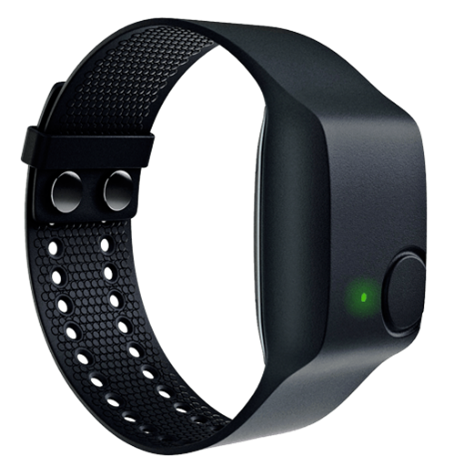
\includegraphics[width=6cm]{img/methods/empaticaE4.png}
\centering
\caption{EmpaticaE4, a wearable device that can record physiological data in real-time.} \label{fig_empatica}
\end{figure}

The Empatica E4 was connected to an Android tablet running the Empatica application, so the researcher could monitor in real-time the data collection. The \ac{EA} app was entirely developed as a set of automated routines in Psychopy, including trainings for the task, synchronization of the triggers with each experimental event and instructions for the users. The timers of each routine were calibrated during the pilot to allow even slower readers to follow up. 

\begin{figure}[h!]
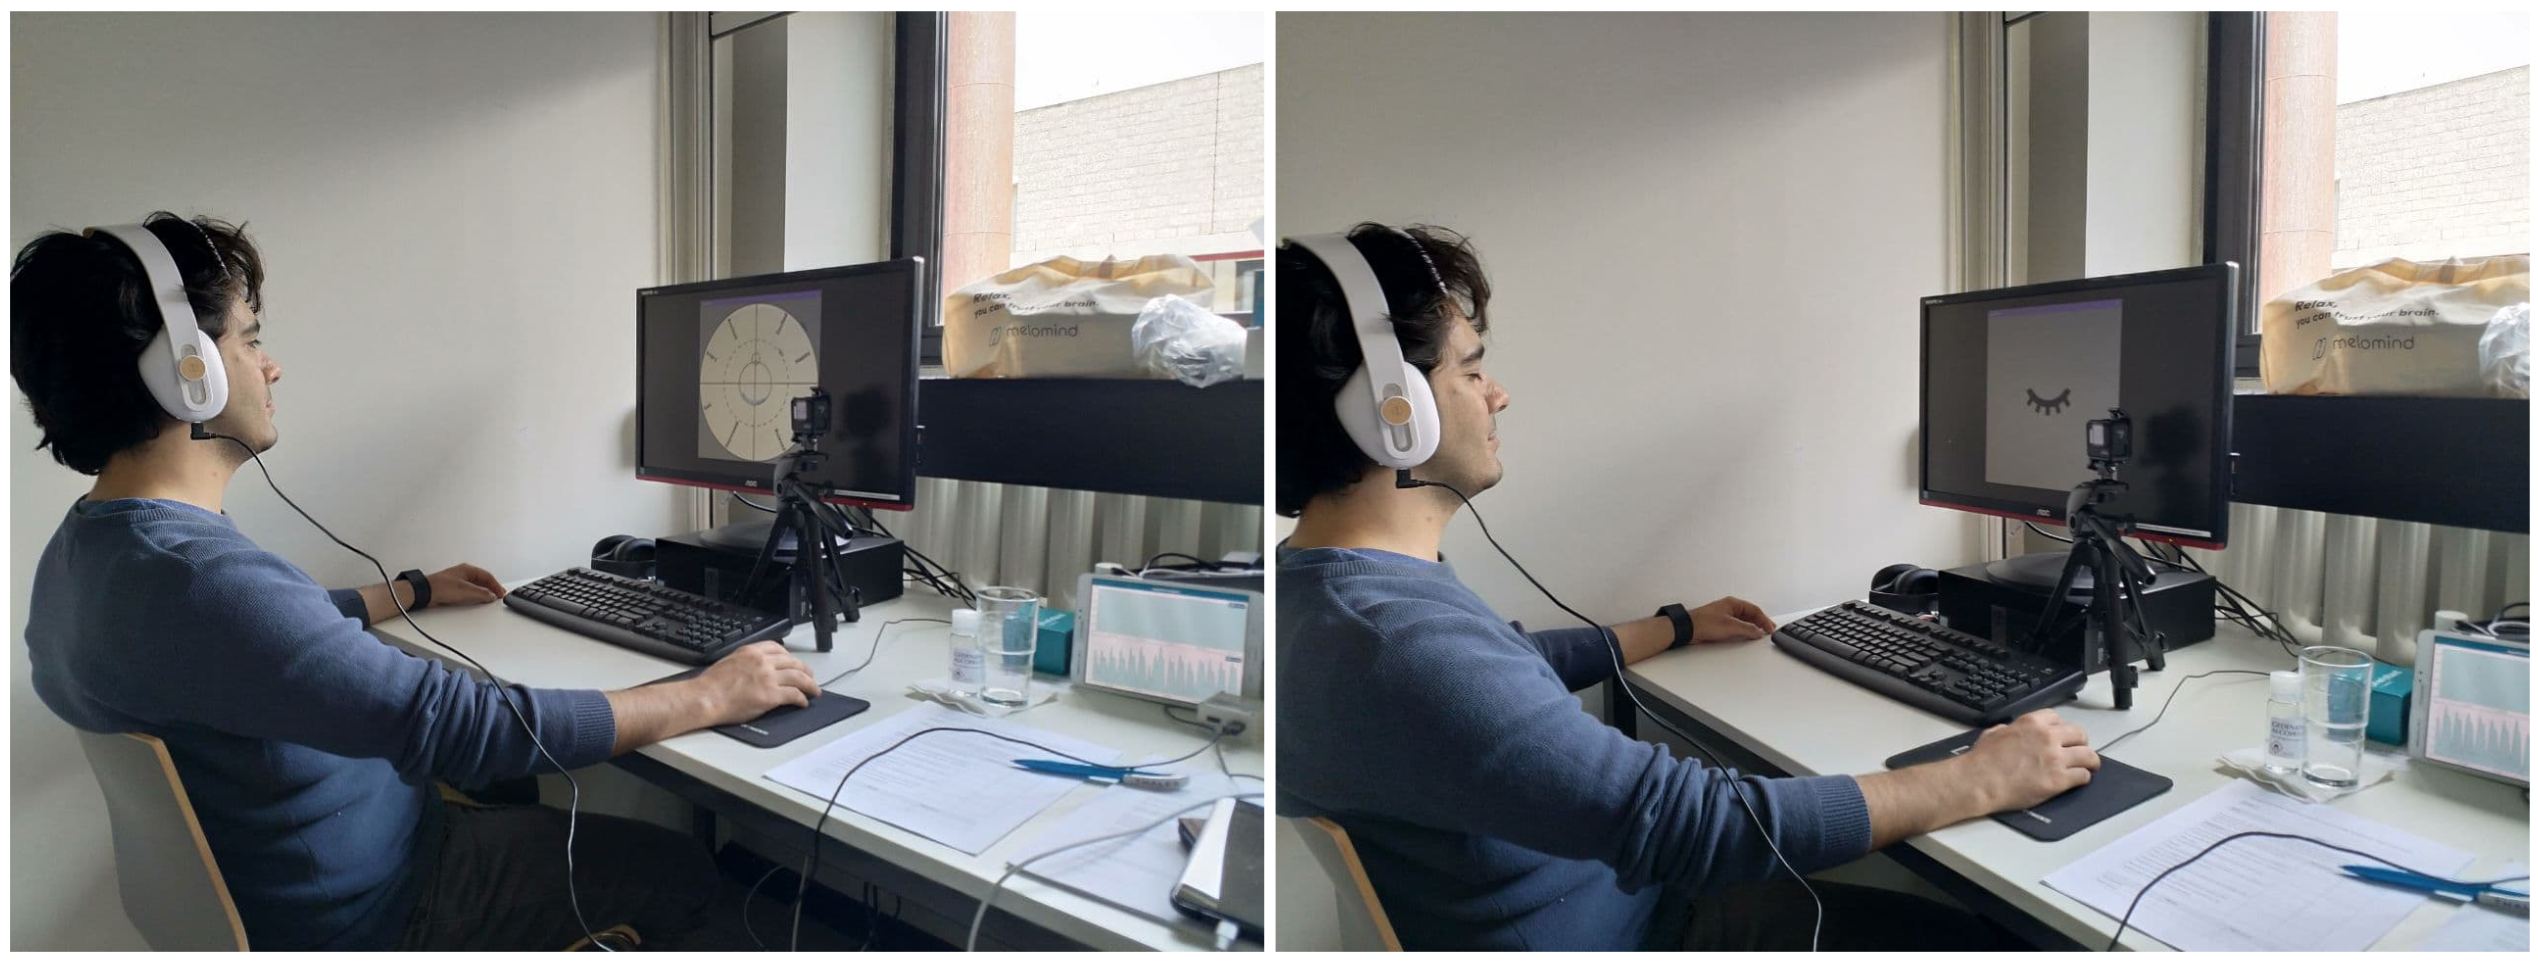
\includegraphics[width=12cm]{img/methods/experimental_setup.png}
\centering
\caption{Experimental setup with Melomind, Empatica E4 and GoProH7. The EA app is running on the monitor, while a participant is annotating emotions using the mouse (on the left) and then following instructions for the next task (on the right).} \label{fig_experimental_setup}
\end{figure}

The participants could interact with the experimental application through an external monitor connected to the researcher’s laptop and an agnostic mouse, although all participants decided to use the right hand. Finally, all the sessions were recorded with a GoPro Hero 7 to monitor accidental events and eventually support the emotion recognition task through facial expressions in a later study. An example of setup for the experiment can be see in Fig. \ref{fig_experimental_setup}. 



\subsection{Procedure}
\label{sec:procedure}
The experiment was conducted in a controlled environment made available by BMS lab at the University of Twente, with a strict protocol for sanitizing the equipment between each session, no direct skin-contact with the researcher during the setup, opening of the air flows every 10-15 minutes and at least 1.5 meters of distance with the researcher during the experimental task.

\begin{figure}[h!]
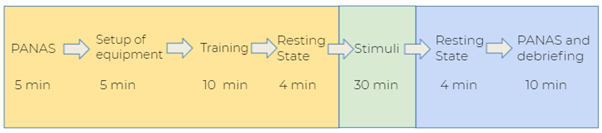
\includegraphics[width=10cm]{img/methods/exp_procedure.png}
\centering
\caption{Scheme of the experimental procedure, estimated to last ~75 minutes.} \label{fig_exp_procedure}
\end{figure}

Upon their arrival, participants were invited to sanitize their hands, to read and sign the informed consent form and then to fill a PANAS questionnaire \cite{watson_development_nodate} as part of myBrainTechnologies standard protocol for experimentation. The PANAS is used to measure the change in positive and negative affects in a specific span of time, from a few minutes up to a few weeks. In this case the span of time is the length of the experiment and researchers at myBrainTechnologies use these questionnaires to evaluate their experimental protocols and eventually support some evidences in their analyses. After the questionnaire, they could start the training session divided into three parts for a total of 10 minutes, without recording any \ac{EEG}. The first part gave some introduction and background about the Valence-Arousal model and allowed them to get some confidence with the annotation GUI. The second part proposed a mix of 4 music excerpts, one for each Valence-Arousal class, and asked them to annotate in real time with the emotions they were feeling. Finally, the third part was a complete simulation of an experimental trial, including instructions, white noises, both listening conditions and ratings. After the training, participants were asked to fit again the device on their head, then the researcher re-positioned the reference and recording electrodes to obtain the best possible quality signal using the \ac{QC} tool of the Acquisier app. The Empatica E4 was then fit on their wrist to allow a precise calculation of heart rate, and finally the Melomind was connected to the laptop through the TriggerBox. Participants were also advised to avoid sudden head movements. Before starting the session, their resting state baseline was recorded, 2 minutes in \ac{EO} condition and 2 minutes in \ac{EC} condition. When they were ready, they could start the session and follow the automated instructions, with the order of conditions determined by their assigned group. Halfway through the session they could take a 5-minute break, look away from the screen and drink some water, but they were not allowed to remove the equipment. After completing the second part of the session, another resting state was recorded with the same settings of the previous one, and then they filled the second PANAS questionnaire. The resting state recordings are also part of the standard myBrainTechnologies protocol to compare the mental changes in the resting states after an experiment and to be used as baseline during \ac{EEG} analysis. For this study only the resting state in the \ac{EC} condition prior to the experimental task was eventually used as recording baseline. At the end of the session all participants were asked to fill a feedback form to briefly evaluate the comfort of the experience, the clarity of the instructions and GUI, any difficulty in the annotation task and to report some behavioral preferences during music listening. Finally, they were debriefed on the purpose of the experiment and dismissed. The total length of the session was of 75 minutes on average, with a maximum of 90 minutes in some cases where the calibration of the equipment was not satisfactory, and the participants were then compensated for their participation.

\section{Data analysis}
\label{sec:data_analysis}
\subsection{Data preparation}
\label{sec:data_preparation}
The first step in the analysis process was to reorganize each participant’s dataset in a systematic collection that could be programmatically parsed. Due to the pseudo-randomization of the classes and the two different conditions, all trials, white noises, and resting states were flagged using an encoded label through the TriggerBox during the experimental phase. The labels were sent using timed events by the \ac{EA} app with a precision in the order of milliseconds. The resulting dictionary of events was used to split the \ac{EEG} recording and extract trials, white noises, and resting states. Each trial was associated with the appropriate label in the format "condition/class\_*\_*" , where condition could be a value between “EO” and “EC” to represent the recording condition, the first * could be a number in the range [1-4] to represent the valence-arousal  class, and the second * a letter between “A” or “B” to represent the order of presentation of a song within each trial. For example, "EO/class\_2\_A" represents the part A of a trial using music from the LAHV class and recording in \ac{EO} condition. In addition, for each \ac{EEG} segment, all the \ac{QC} labels were saved for later use in the preprocessing pipeline (see Chapter \ref{sec:automated_pipeline}). Then another dictionary containing the order of presentation of the classes was used to associate the metadata saved by the \ac{EA} app, namely the valence-arousal annotations and the familiarity/liking scores for each song, to the respective entry in the newly organized dataset. During the experiment sessions, some rare bugs in the recording application caused brief interruptions in the recording or the failure to register triggered events. For this reason, a total of 6 participants who had missing parts in their \ac{EEG} recordings or did not have the dictionary of events were excluded for further analysis. Their data could still be utilized in future studies by synchronizing the splitting functions with the timestamps saved in the metadata, but because of the time cost, it was decided to exclude them for the current research.

\subsection{Automated Pre-processing Pipeline}
\label{sec:automated_pipeline}
Given the goal of estimating the performances of a real-time oriented model, the pre-processing of the data had to consist of a lightweight and automated process that could be integrated in an application at some point. Consequently, more run-in tools like EEGLab and PREP \cite{bigdely-shamlo_prep_2015}, both based on the MATLAB programming language and very popular for offline analysis, were discarded in favor for more real-time oriented tools. Therefore, the \ac{AuPP} was implemented as a combination functions of the open-source Python library MNE\footnote{https://mne.tools/stable/index.html}  and the \ac{SPT} from myBrainTechnologies, a closed-source library that is more suitable to handle the proprietary data format of Melomind. After loading each participant’s prepared dataset, the \ac{AuPP} splits the signal in time windows of 5 seconds, removes the DC offset, applies a notch filter to remove power-line noise in the 50Hz and the 100Hz frequency bands, then applies a band-pass filter in the range 0.1Hz - 30Hz to remove slow and possibly large amplitude drifts and some movement artifacts outside of the frequency bands of interest (Fig. 22). Unfortunately, this light preprocessing is not suitable to remove most of the muscular artifacts, especially those generated by ocular movements that are frequently present in the frontal electrodes. In addition, having two electrodes hinders artifact detection using more sophisticated signal processing algorithms like \ac{ICA} and \ac{PCA}, that require a higher number of electrodes to effectively separate the signal in components and identify artifacts. To deal with artifacts, the \ac{AuPP} features two methods that can be used independently or in conjunction.

\begin{figure}[h!]
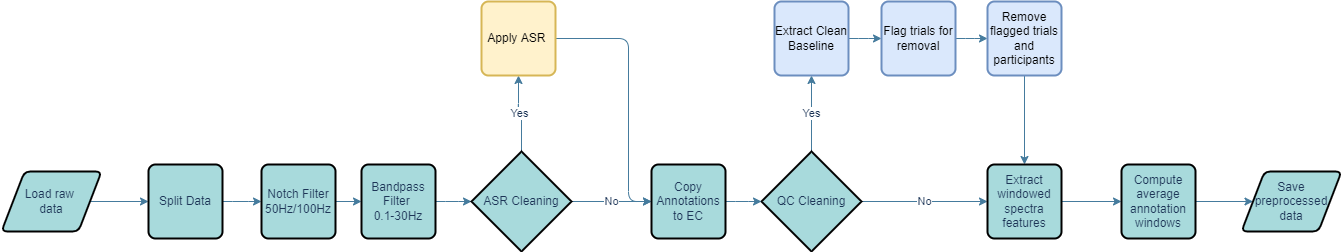
\includegraphics[width=15cm]{img/methods/preprocessing_pipeline.png}
\centering
\caption{Flowchart representing the preprocessing steps of the AuPP.} \label{fig_prep_pipeline}
\end{figure}

The first one is  \ac{ASR}, available in the open-source MEEGkit\footnote{https://nbara.github.io/python-meegkit/index.html}  library, that automatically tries to clean the signal by removing transient and large-amplitude artefacts. The second one is a custom method called \ac{QIRem}, implemented for this study, and based on the \ac{QC} proprietary classification-based method developed by myBrainTechnologies. The \ac{QC} algorithm has been developed to support researchers in real-time visual assessment of the quality of the signal \cite{grosselin_quality_2019}, and for each second of recording it assigns a label representing the quality of the signal as follows:
\begin{itemize}
\item 	Low Quality: LOW-Q = -1 and 0. 
\item 	Medium Quality with muscular artefacts: MED-MUSC = 0.25. 
\item 	Medium Quality: MED-Q = 0.5. 
\item     High Quality: HIGH-Q = 1.
\end{itemize}

The \ac{QIRem} method takes the \ac{QC} labels and redistribute them on a simpler scale from 0 to 1, where 0 corresponds to LOW-Q, 0.5 corresponds to MED-MUSC-Q and MED-Q and 1 corresponds to HIGH-Q, and then for each 5 seconds time window it calculates an average of the \ac{QC} labels.

\begin{figure}[h!]
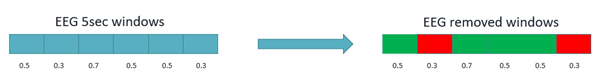
\includegraphics[width=15cm]{img/methods/qirem_example.png}
\centering
\caption{Example of how QIRem flags bad segments flagged for removal.} \label{fig_qirem_example}
\end{figure}

If the average is below a specified \emph{threshold} parameter, the EEG split is removed from the dataset (Fig. \ref{fig_qirem_example}). After removing all the contaminated splits if the dataset has lost more than the percentage of data  amount specified by the \emph{allowed loss} parameter, the entire participant’s dataset is flagged for exclusion from the analysis. During the tuning of the \ac{AuPP}, it was finally decided to avoid using \ac{ASR} to clean the signal, because it requires to be trained on a sufficiently clean segment of signal, unfortunately not guaranteed to exist for all subjects, and most often resulted in very aggressive cleaning that would flatten the signal (Fig. \ref{fig_asr_example}).

\begin{figure}[h!]
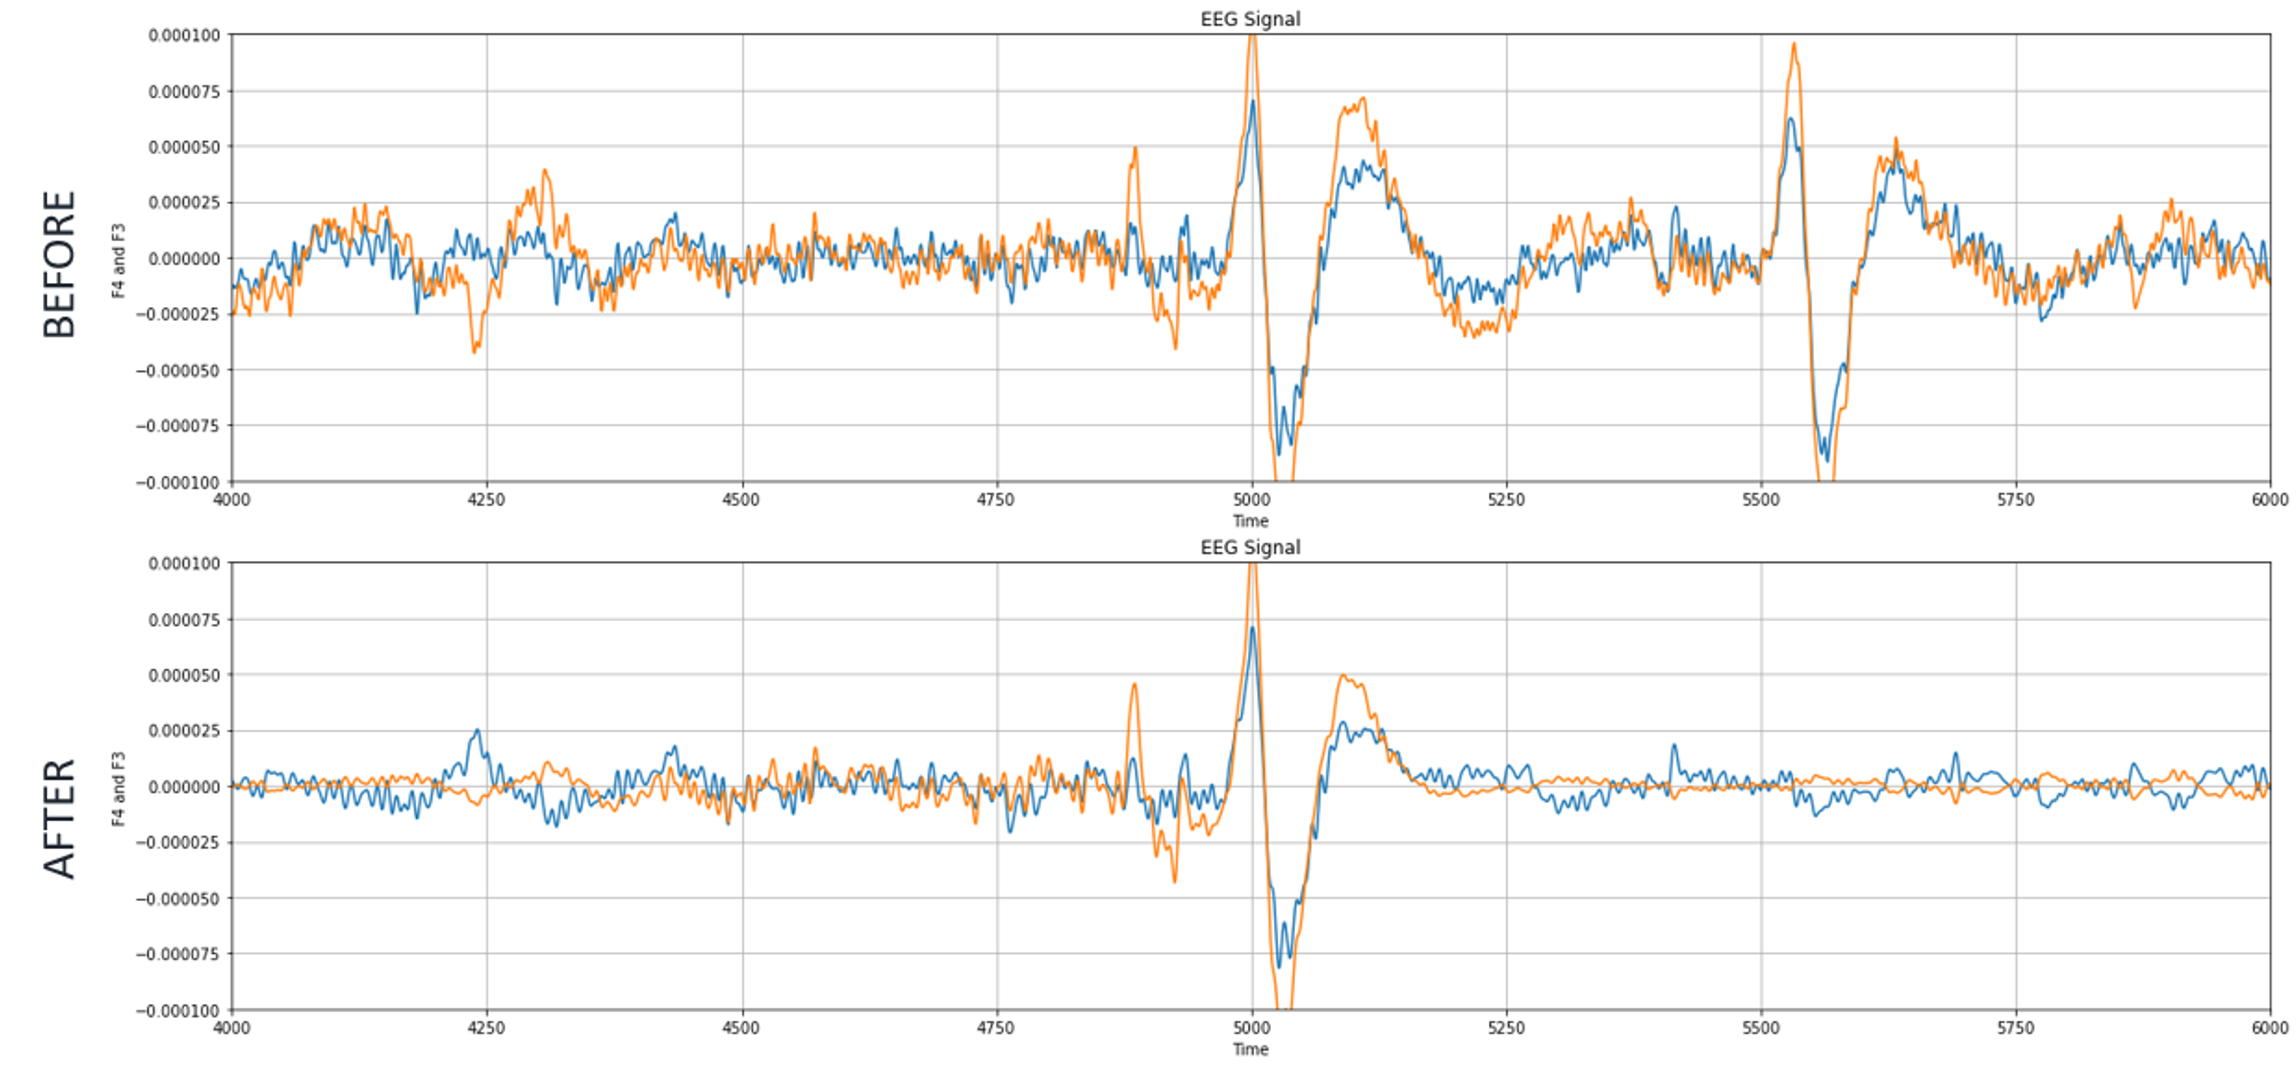
\includegraphics[width=15cm]{img/methods/asr_example.png}
\centering
\caption{Examples of the effects of ASR on the signal.} \label{fig_asr_example}
\end{figure}

The \ac{QIRem} method was setup with \emph{threshold} set to 0.5 and \emph{allowed loss} set to 0.25, meaning that the average quality of each time window had to be equal or above 0.5 in the simplified scale and that at most 25\% of data could be pruned before flagging the entire dataset for exclusion. With the current configuration, 10 participants were excluded from further analysis, hence the reason why the threshold was kept around medium quality (0.5), allowing some artefacts to persist in the data. This approach is a compromise choice that carries three main problems that must be addressed in future studies:
\begin{itemize}
\item 	Very aggressive: bad quality data are not cleaned, but removed instead, possibly losing meaningful information and control over the distribution of the class labels.
\item 	Exclusive: 10 out of 39 participants were excluded from analysis, which summed up to those excluded for other reasons is more than 1/3 of the entire experimental dataset.
\item 	Not Optimized: one limitation of the Quality Checker algorithm is that it was trained for the consumer use on Melomind with electrodes placed on the parietal area of the scalp (P3, P4), so while able to discriminate good and bad quality segments of signal, it has no specific label for ocular artifacts. An upgraded version is under the work to provide classification of these artifacts.
\end{itemize}

\subsection{Features Computation}
\label{sec:features_computation}
To compute the spectral features, the \ac{PSD} of each 5 seconds window of the \ac{EEG} signal was extracted and filtered for theta, alpha and beta frequency band using the \ac{SPT} wrapper for the \ac{FFT}. Before computing features, the time-frequency power was normalized using the decibel conversion method as described by M. X. Cohen \cite{cohen_analyzing_2014}. Time-frequency power follows a 1/f shape function, meaning that frequency spectrum tends to show decreasing power at increasing frequencies, \ac{EEG} included. Consequently, there are 4 main limitations:


\begin{enumerate}
\item 	Difficulty in making power comparisons across such bands. Raw power values change in scale as a function of frequency, meaning that lower frequencies (Delta, Theta) will show larger effect than higher frequencies in terms of overall magnitude.
\item 	Aggregation of subject-independent effects will not yield good results because of differences influenced by skill thickness, sulcal anatomy, cortical surface, recording environment or other internal and external factors.
\item 	Task-related changes in power can be tainted by background activity, particularly for frequencies that tend to have higher power, especially during baseline periods (Alpha).
\item 	Raw powers do not follow a normal distribution because they cannot be negative, and they are strongly positively distorted.
\end{enumerate}
Using decibel conversion, which is an expression of power as the ratio between strength of one signal (frequency-band-specific-power) and the strength of another signal (a baseline level of power in the same frequency band).
\[dB_{tf} = 10log10 \left(\frac{activity_{tf}}{\overline{baseline_{tf}}} \right)\]
The scale and interpretation of frequency-band-specific power becomes the change in power relative to the baseline. Any frequency-band-specific activity constant over time will be removed, including background activity. As a baseline for normalization, the resting state in the \ac{EC} condition was used, to prevent ocular artifacts from contaminating the trials. The baseline resting state, previously divided in 5 seconds time window, and pre-processed together with the other trials, was pruned from low quality segments using the \ac{QIRem} function and then averaged across all the time windows, for each channel. The main advantages obtainable by normalizing the date are the following: 

\begin{itemize}
\item 	All power data are re-scaled to the same scale and thus can be compared visually and statistically
\item 	Normalization computed in respect to a pre-trial baseline enables to disentangle time-frequency dynamics from background or task-unrelated dynamics
\item 	All power results are in a common and easily numerically interpretable metrics
\item 	Parametric statistical analysis is appropriated to use (for baseline-normalized power data normally distributed) and quantitative group-level analyses and integration with other data (behavioral performance, questionnaires) is facilitated. 
\item 
\end{itemize}
The features extracted include the neuromarkers described in Chapter \ref{chap:background} and additional properties of the power spectrum that could strengthen the models’ ability to discriminate emotional dimensions. It was decided in a later stage to use these properties of the raw signal because they could be conveniently extracted using the \ac{SPT} and potentially make up for information lost during the computation of the neuromarkers.
For each 5s time window the following measurements were computed and stored, for a total of 40 features among the two channels to be used in classification:
\begin{enumerate}
\item 	Normalized power in Theta, Alpha and Beta frequency bands
\item 	Approach-Withdrawal Index 
\item 	Frontal-Midline Theta Index
\item 	Spectral Asymmetry Indexes
\item 	Skewness of the power in Theta, Alpha and Beta frequency bands
\item 	Kurtosis of the power in Theta, Alpha and Beta frequency bands
\item     Standard deviation of the power in Theta, Alpha and Beta frequency bands
\item 	Ratio of the power in Theta, Alpha and Beta frequency bands
\item 	Relative spectral difference of the power in Theta, Alpha and Beta frequency bands
\end{enumerate}


\begin{figure}[h!]
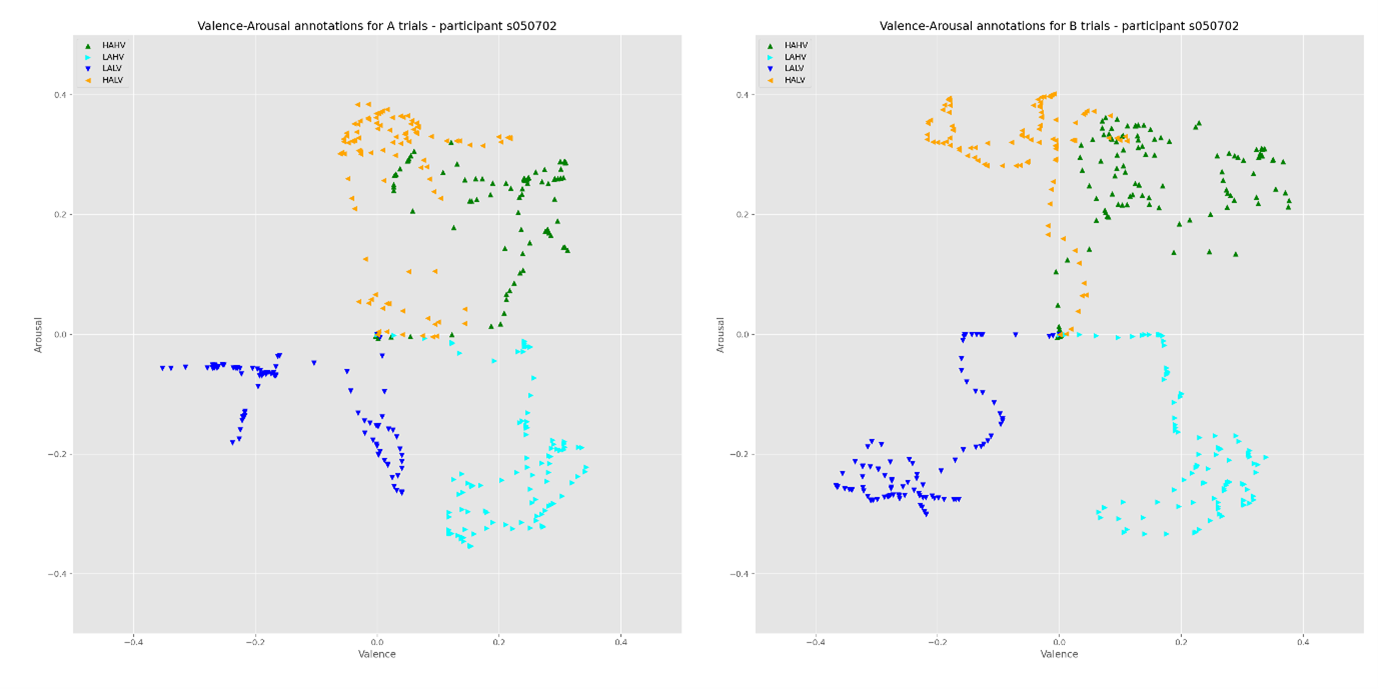
\includegraphics[width=15cm]{img/methods/example_avg_annotations.png}
\centering
\caption{Example of annotations of a single participant for all trials. The labels are color coded according to the pre-labelled VA class of each song.} \label{fig_avg_annotations}
\end{figure}

Finally, the raw VA annotations (Fig. \ref{fig_avg_annotations}) were averaged for each time-window and then converted into positive labels whether the average was positive, or negative labels otherwise. Consequentially, each time window was labelled twice: first as HA or LA (High/Low Arousal), and then as HV or LV (High/Low Valence). The union of the two labels generates one of the class labels of the Valence-Arousal quadrant that represent the emotion elicited in that specific time window, according to the notation proposed by Koelstra et al. \cite{koelstra_deap_2012} (see Chapter \ref{sec:stimuli}). In some studies, the notation for valence is defined as PV and NV (Positive/Negative Valence), which is better aligned with the etymology of positive and negative emotions. The labels were also copied for each song from the \ac{EO} listening condition to the respective \ac{EC} listening condition.

\subsection{Classification}
\label{sec:classification}
The classification pipeline was implemented using the open-source Python library Scikit-Learn\footnote{https://scikit-learn.org/stable/index.html}. Multiple experiments were conducted with two supervised learning models, \ac{SVM} and \ac{MLP}. These models are a popular choice for the Emotion-Recognition task thanks to their relative simplicity yet their superior capacity to handle not linearly separable data compared to statistical linear models (see Chapter \ref{sec:classification_emotions}). The \ac{SVM} architecture was defined using RBF kernel, that usually grants better accuracy, and it is relatively easy to calibrate, and decision function one-vs-one for binary classification and one-vs-rest for multi-class classification. The architecture for \ac{MLP} was based on the LBFGS optimizer, a quasi-Newtonian method, that is more suitable for small datasets and can converge faster with better perforances and \emph{ReLU} was chosen over \emph{TanH} as activation function because it reduces the impact of vanishing gradients, even if no substantial difference was observed while testing both. The problem has been set as a separate binary classification of Arousal and Valence using a subject-dependent strategy, similarly to most related studies. As explained in the Section \ref{sec:intermediate_experiments}, during the intermediate experiments the listening condition did not reveal significant differences in the classification performances, therefore all the trials of each subject were later unified under a third condition named “EO\&EC” to take advantage of the greater amount of data-points. Then, from each subject dataset, a total of 40 previously computed features were loaded in the classification pipeline.
\begin{figure}[h!]
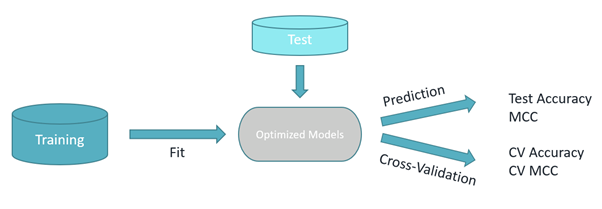
\includegraphics[width=12cm]{img/methods/data_split_strategy.png}
\centering
\caption{Approach used to compute Test Accuracy, MCC, CV Accuracy and CV MCC with separate splits of data.} \label{fig_data_split_strategy}
\end{figure}
To begin with, the data were split into a training dataset and a test dataset in 80:20 proportion and scaled using MaxAbsScaler, that re-scales the data to its maximum absolute value without shifting or centering it, thus preserving any sparsity.\ac{PCA} was used to identify the features contributing for the 95\% of the variability of the dataset and projecting them on a lower dimensional space, reducing the dimensionality to ~12 components and greatly reducing the overall computation time, often referred to as \emph{curse of dimensionality}. After applying \ac{PCA}, the training dataset was used to tune the best hyper-parameters each classifier, respectively \emph{C} and \emph{Gamma} for \ac{SVM} and \emph{Alpha} and \emph{Hidden Layer Sizes} for \ac{MLP}, using GridSearch with a K-Fold Cross-Validation strategy, k=5 (see Fig, \ref{fig_data_split_strategy}). Finally, the tuned classifiers were trained with K-Fold Cross Validation \ac{LOBO} for testing, and the relevant score metrics were collected.

\subsection{Intermediate experiments}
\label{sec:intermediate_experiments}
The classification problem was initially addressed as a binary classification problem for Arousal and Valence and then as a multi-class classification problem for Valence-Arousal. During the initial experimentation phase, these models were manually tuned and studied keeping the listening condition separated and then adding a third condition defined as EO\&EC, composed by data from both listening conditions joint together. To explore each condition and each type of model, a binary classifier for Arousal, a binary classifier for Valence and a multi-class classifier for Valence-Arousal were trained, following both subject-dependent and subject-independent strategy, for a total of 36 possible combinations. All the other hyper-parameters were initially manually tuned and kept identical for each classifier (see Appendix \ref{sec:appendix_A3.1}). The first full-scale experiment was launched with subject-dependent strategy and to reduce the dimensionality of the data, the 5 most relevant features were selected using forward \ac{SFS} with cross-validation to select the features most contributing to the variability of the data and using them to train each subject’s classifiers with cross-validated scores. Consequently, the selected features were ranked by adoption rate among all participants (see Appendix \ref{sec:appendix_A3.1}) and appointed as TOP5 features. It should be emphasized that this operation was computationally intensive and took several hours to complete, underlying the necessity for a better approach to envision a real-time application. Another subject-dependent experiment was run, this time using the same pre-selected TOP5 features for each participant, followed by a subject-independent experiment with the same configuration with cross-validation and \ac{LOSO}. The results of all experiments have been collected and averaged (see Appendix \ref{sec:appendix_A3.1}, \ref{sec:appendix_A3.2}, \ref{sec:appendix_A3.4}). A few observations were made that led to further investigation and the search for a better approach:
\begin{itemize}
\item 	\ac{EC} and \ac{EO} conditions did not show significant differences in performance, suggesting that the study could continue using just the EO\&EC condition, greatly reducing computation time and simplifying the analysis.
\item 	The multi-class classifiers for \ac{VA} reported the worst performances, thus was discarded to focus the efforts on optimizing the binary classifiers.
\item 	Many datasets were highly unbalanced in the distribution of the labels among the four \ac{VA} classes and both \ac{MLP} and \ac{SVM} struggled to discriminate positive and negative class, with \ac{SVM} always default guessing the majority class.
\item 	Subject-Independent performance always resulted very close and sometimes worse than default guessing the majority class.
\item 	Selecting the average TOP5 features among all participants is idealistically a good choice for a subject-independent strategy, but given the more promising subject-dependent results, this approach is at best losing data variability for some of the subjects and at worse using the least contributing features for some others.
\end{itemize}

Further investigation in the subjects labelling behavior and in the models’ predictions (see Appendix \ref{sec:appendix_A3.4}) led to the decision to optimize the strategy in function of subject-dependent classification.

\subsection{Unbalanced labelling}
\label{sec:unbalanced_labelling}
The stimuli were selected to elicit a wide as possible range of emotions to cover evenly the Valence-Arousal quadrants. However, when selecting music that has been pre-labelled with the average opinion of hundreds of annotators, there is always a possibility that part of the population disagrees. These subjects are not per se “bad annotators”, but their personal taste and perception lies outside of median. The distribution of labels across all subjects in Figure \ref{fig_labels_distribution} also reveals that positive classes are in general the most reported, with HAHV and LAHV taking absolute lead, and corresponding to emotions very common during the music listening experience: excitement, happiness, satisfaction, calm etc.

\begin{figure}[h!]
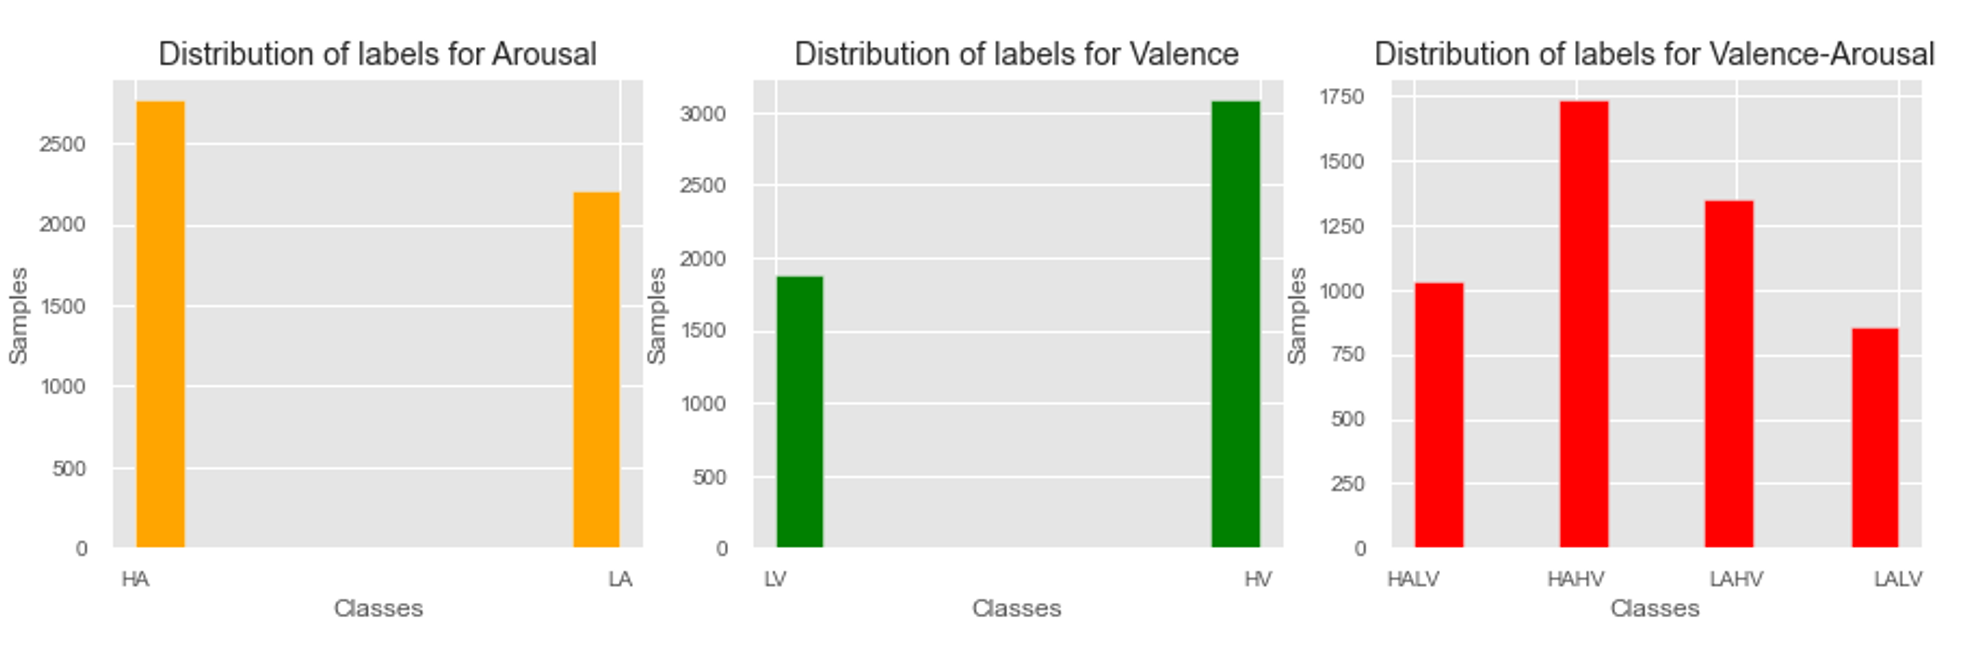
\includegraphics[width=12cm]{img/methods/labels_distribution.png}
\centering
\caption{Distribution of arousal, valence, and Valence-Arousal labels across all subjects.} \label{fig_labels_distribution}
\end{figure}

Furthermore, the personal perception of a subject can be heavily biased by external factors such as memories, genres preferences or unexpected events occurred over the day that are outside of the experiment control capabilities. In some cases, this led to very extreme distributions of data (Fig. \ref{fig_unbalanced_example}).

\begin{figure}[h!]
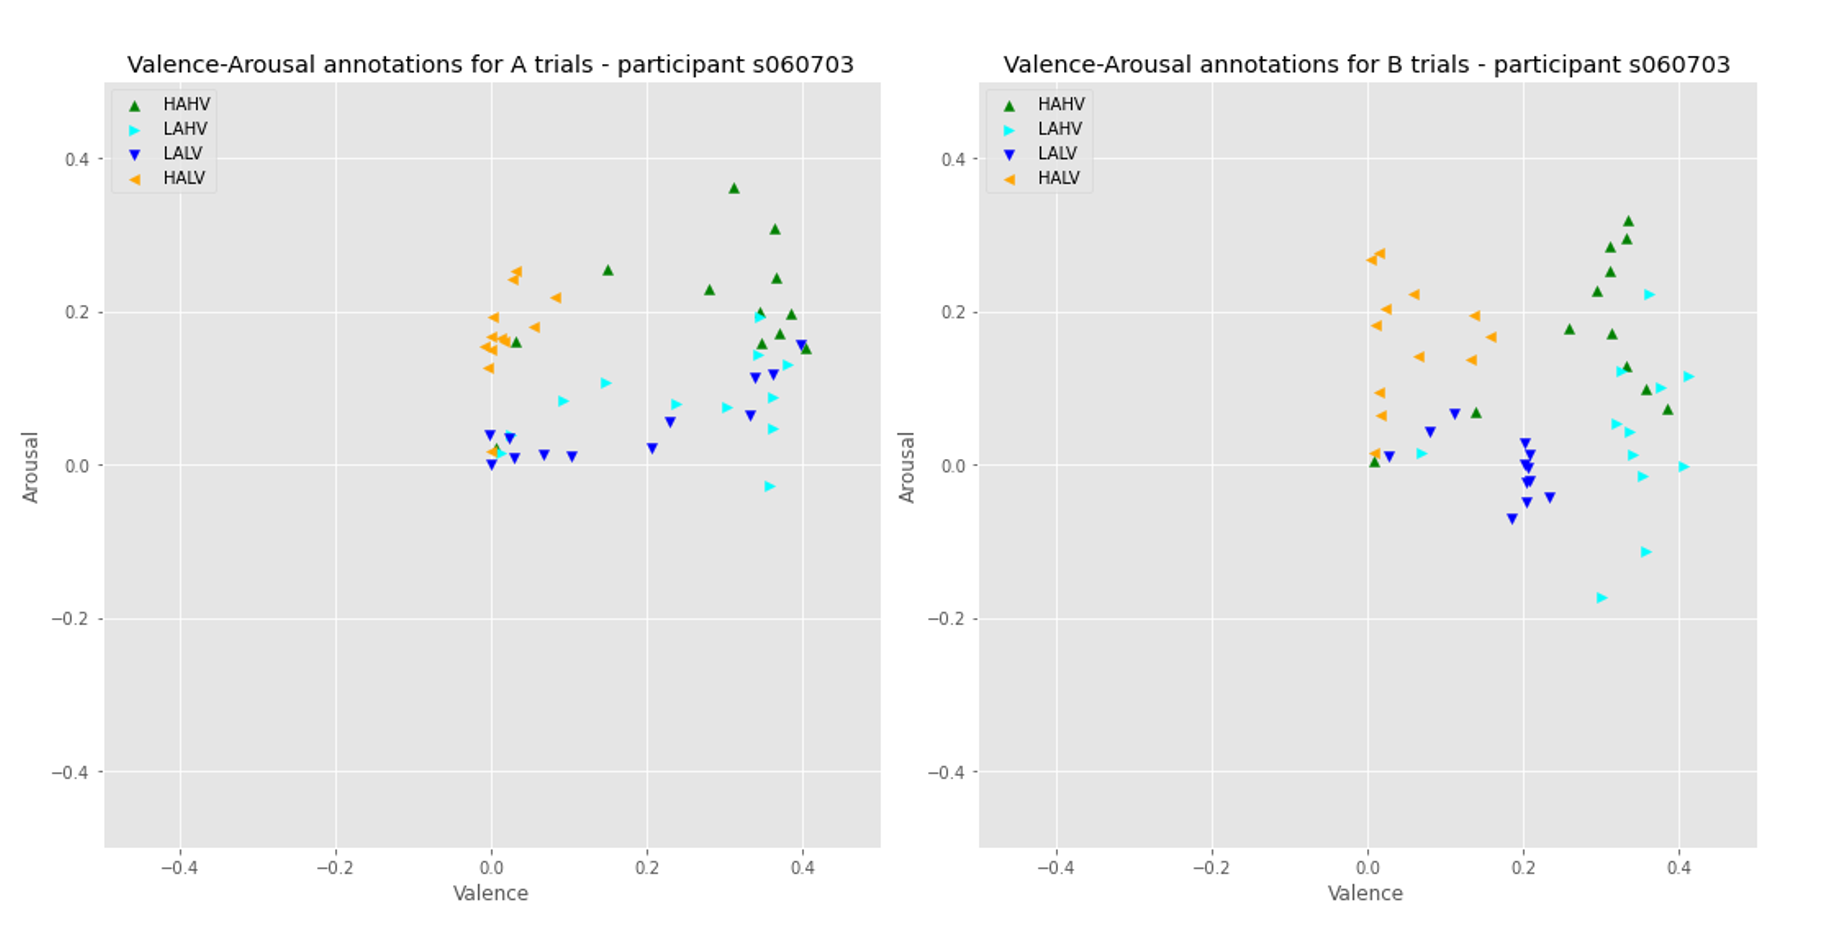
\includegraphics[width=12cm]{img/methods/unbalanced_example.png}
\centering
\caption{Annotations averaged over a 5 second window for a subject with unbalanced dataset. The labels are color coded according to the pre-labelled VA class of each song.} \label{fig_unbalanced_example}
\end{figure}

Although just a few data points of this subject lie in the negative spectrum of Arousal and Valence, the continuous annotations allow to capture them while discrete annotations at the end of each song might have ended up all in the HAHV class, thus hindering any classification. However, a classifier trained to obtain the maximum accuracy would always overfit and opt to classify the majority class, misleading the interpretation of its performances. 

\subsection{Optimizations}
\label{sec:optimizations}
All the problematics were addressed before proceeding with the final experiment. First, the dimensionality of the features was reduced using \ac{PCA} to select the 95\% most contributing components, greatly reducing the computational time and the risk of excluding meaningful features. Then \ac{MCC} \cite{matthews_comparison_1975} was introduced as scoring parameter to provide better interpretability of the accuracy scores. The \ac{MCC} is a correlation coefficient between the observed and predicted binary classification and is defined by the following formula: 
\[MCC = \frac{TP \times TN - FP  \times FN}{\sqrt{(TP + FP)(TP + FN)(TN+ FP)(TN + FN)}}\]
The \ac{MCC} value ranges between -1 and +1, where +1 represents a perfect prediction, 0 a random prediction and -1 and inverse prediction. Unlike the F1 score, that is the harmonic mean of precision and recall, the \ac{MCC} considers all the four quadrants of the confusion matrix of a prediction, making it a more reliable measure for the learning performances of a model for binary classification, even when the dataset is unbalanced \cite{chicco_advantages_2020}. The large number of factors that may hinder the Emotion-Recognition task are reflected in the large variability of the classification results across subjects and thus using solely the accuracy to measure the performances is not optimal and more studies \cite{thammasan_multimodal_2017, keelawat_comparative_2021} now relying on \ac{MCC} score’s reliability to explain the learning capabilities of their models. To optimize the models for the subject-dependent strategy, GridSearch was used with K-Fold Cross-Validation on the training split of each subject dataset to find the configuration that would yield the highest \ac{MCC} score (see Fig. \ref{fig_scheme_data_splitting}). 

\begin{figure}[h!]
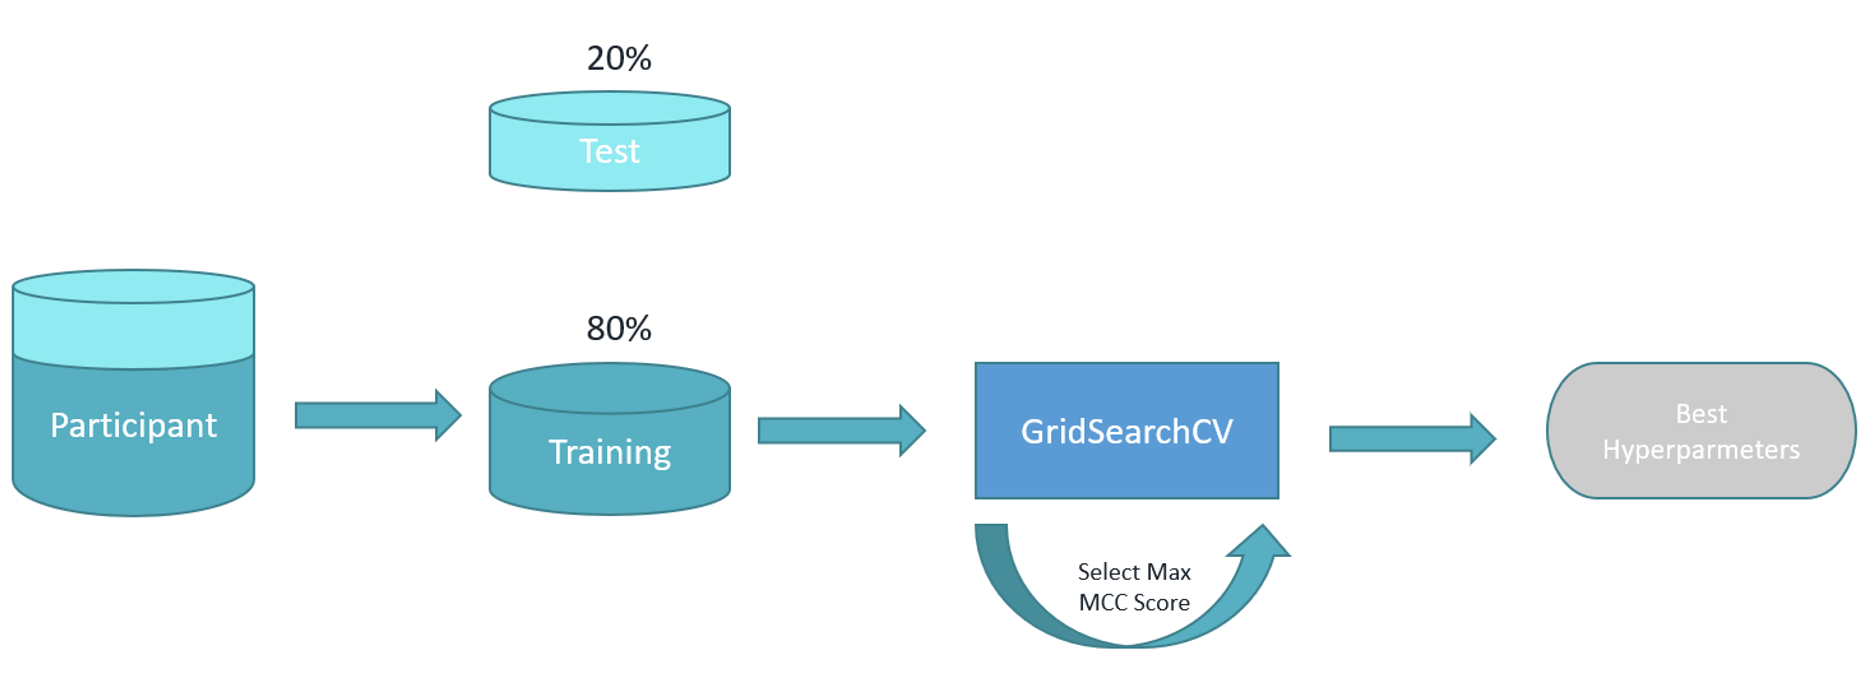
\includegraphics[width=12cm]{img/methods/scheme_data_splitting.png}
\centering
\caption{Scheme of data splitting strategy for cross-validated GridSearch optimization.} \label{fig_scheme_data_splitting}
\end{figure}

In addition, \ac{SVM} models were also initialized with the weights of each class based on the distribution of the labels. Currently there is a known limitation in the Scikit-learn library, as it does not seem to support custom loss functions to optimize scoring parameters other than accuracy, a missing feature reported by users of the library \cite{martin_stacked_nodate, noauthor_please_nodate}. Consequently, when feeding \ac{MCC} as scoring parameter, it only means that after optimizing accuracy for all possible configurations, the configuration with highest \ac{MCC} is selected. Two scoring strategies for GridSearch were tested in the intermediate experiments:
\begin{itemize}
\item 	Maximization of \ac{MCC} score, defined as “Max MCC” strategy
\item 	Maximization of Accuracy score, defined as “Max Accuracy” strategy
\end{itemize}
Maximising accuracy scores is often desirable in machine learning because it gives a clear idea of a model's ability to predict a class. A "good" accuracy in most cases should be above 90\%, while for an optimal score should be above 99\%. However, given the presence of many unbalanced datasets in the current research, the "Max Accuracy" strategy for GridSearch generated more often over-fitted models that would have higher accuracy, at the cost of never predicting the minority class, especially with \ac{SVM} classifiers (see Appendix \ref{sec:appendix_A3.5}). With \ac{MLP} classifiers this phenomenon was less evident, also because they already produced a larger number of over-fitted and under-fitted models than their \ac{SVM} counterparts, however in spite of using the same strategy and \ac{MCC} as principal metric to show evidences of learning capabilities, the "Max MCC" strategy was chosen to proceed with the final experiment.

\iffalse
\section{Better learning or better accuracy}
\label{sec:better_learning_accuracy}
The purpose of this intermediate experiment was to compare the scoring strategies; however, it is important to underline that the loss function implemented in the scikit-learn library for GridSearch is chosen to optimize accuracy and only then the scoring parameter is used to select the best configuration. The results of subject-dependent arousal classifications are reported in Table 3, and they are not significantly different from the previous experiment. However, the highest consistent accuracy score using \ac{MLP} is 77\% with \ac{MCC} score of 0.53. Furthermore, it is possible to notice an increased number of negative \ac{MCC} and \ac{CV MCC} scores, and for \ac{MLP} the best performing models are not entirely consistent with the previous experiment.

\begin{table}[h!]
  \caption{Arousal classification results using Accuracy as scoring parameter for GridSearch. The 5 best performing models in terms of accuracy and MCC score are highlighted in blue, the models with MCC <= 0 and CV MCC <= 0 are highlighted in orange and yellow, respectively.}
  \label{tbl:arousal_max_acc_results}
  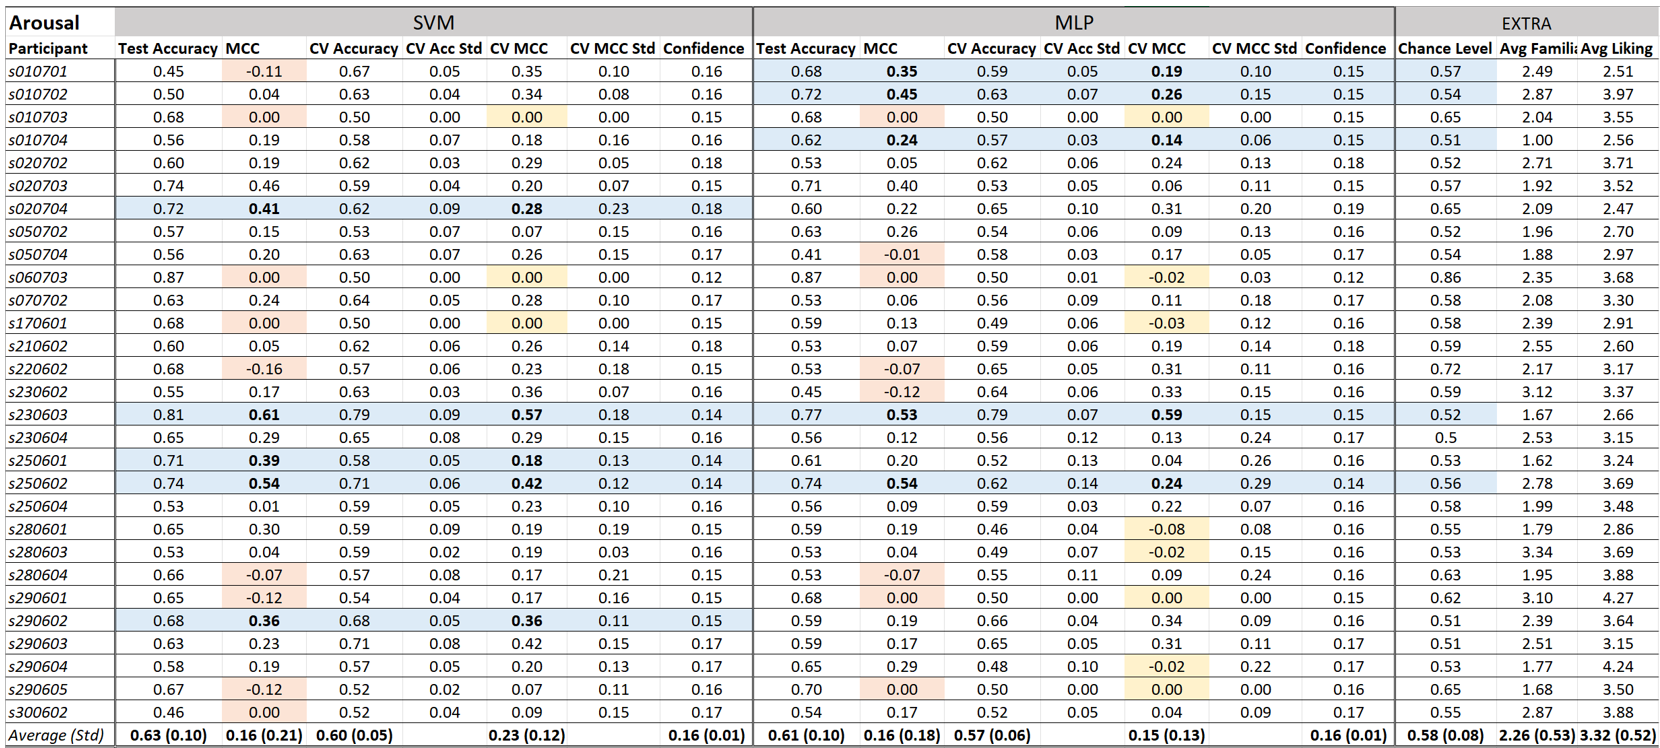
\includegraphics[width=\linewidth]{img/results/arousal_max_acc_results.png}
\end{table}

For valence classification the average test score is slightly higher for both \ac{SVM} and \ac{MLP}, but the highest accuracy score for \ac{MLP} reaches 90\% with \ac{MCC} score of 0.36. For \ac{SVM} the highest accuracy score is 80\% with \ac{MCC} score of 0.11. These highest accuracy scores are not consistent with the previous experiment and the relatively lower associated \ac{MCC} scores can be explained by the different scoring strategy.

\begin{table}[h!]
  \caption{Valence classification results using Accuracy as scoring parameter for GridSearch. The 5 best performing models in terms of accuracy and MCC score are highlighted in blue, the models with MCC <= 0 and CV MCC <= 0 are highlighted in orange and yellow, respectively.}
  \label{tbl:valence_max_acc_results}
  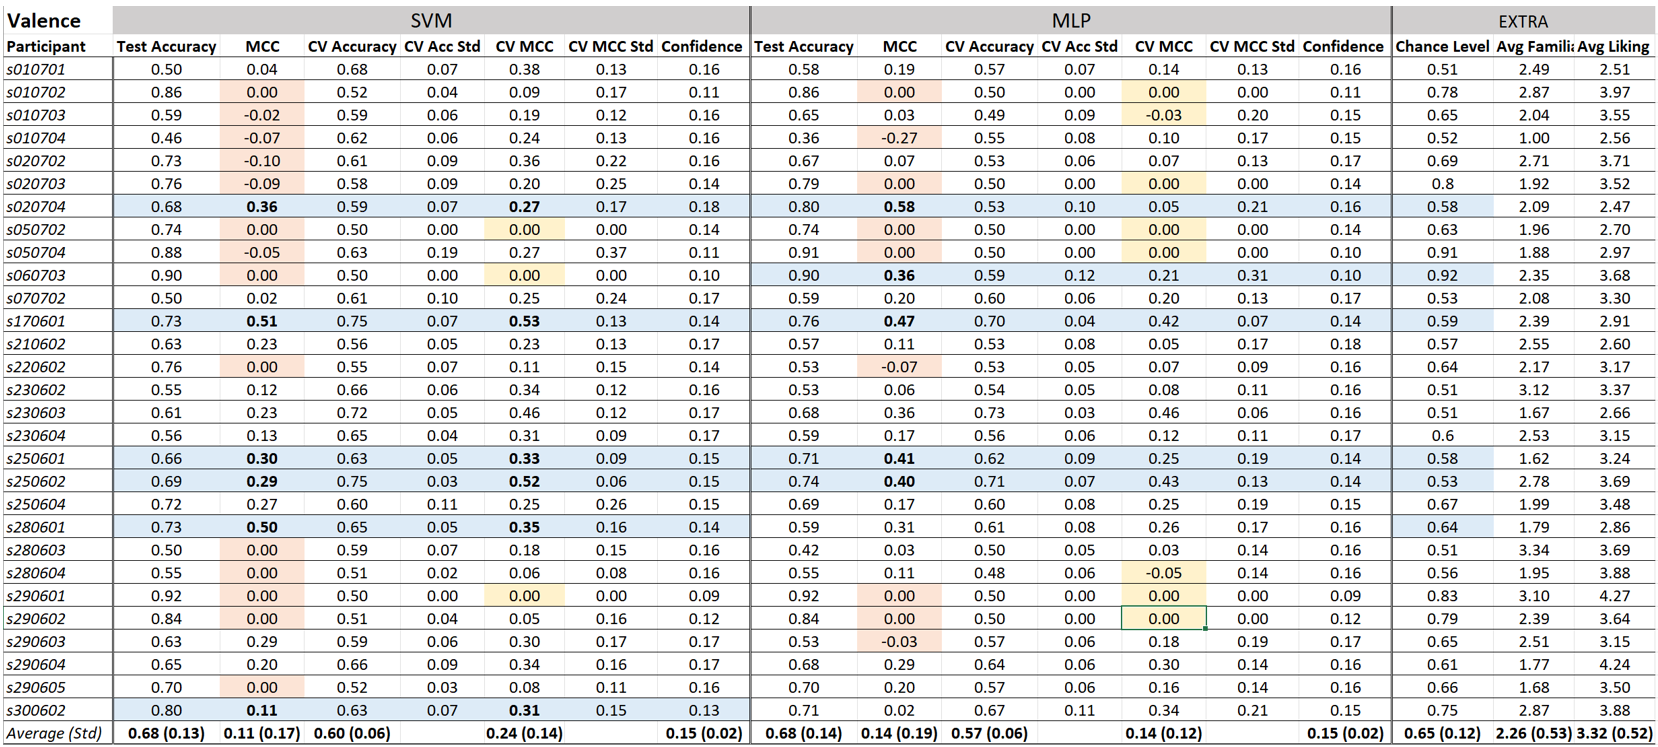
\includegraphics[width=\linewidth]{img/results/valence_max_acc_results.png}
\end{table}

Overall, it is also noticeable that an increased number of models is not learning, either because of over-fitting or under-fitting. This is particularly evident for arousal classification. This can be observed in the plots in Fig. \ref{fig:arousal_strategy_comparison} and Fig. \ref{fig:valence_strategy_comparison}, in which the number of models scoring 0 or less in \ac{MCC} and \ac{CV MCC} scores is compared between both strategies, for arousal and valence respectively.

\begin{figure}[h!]
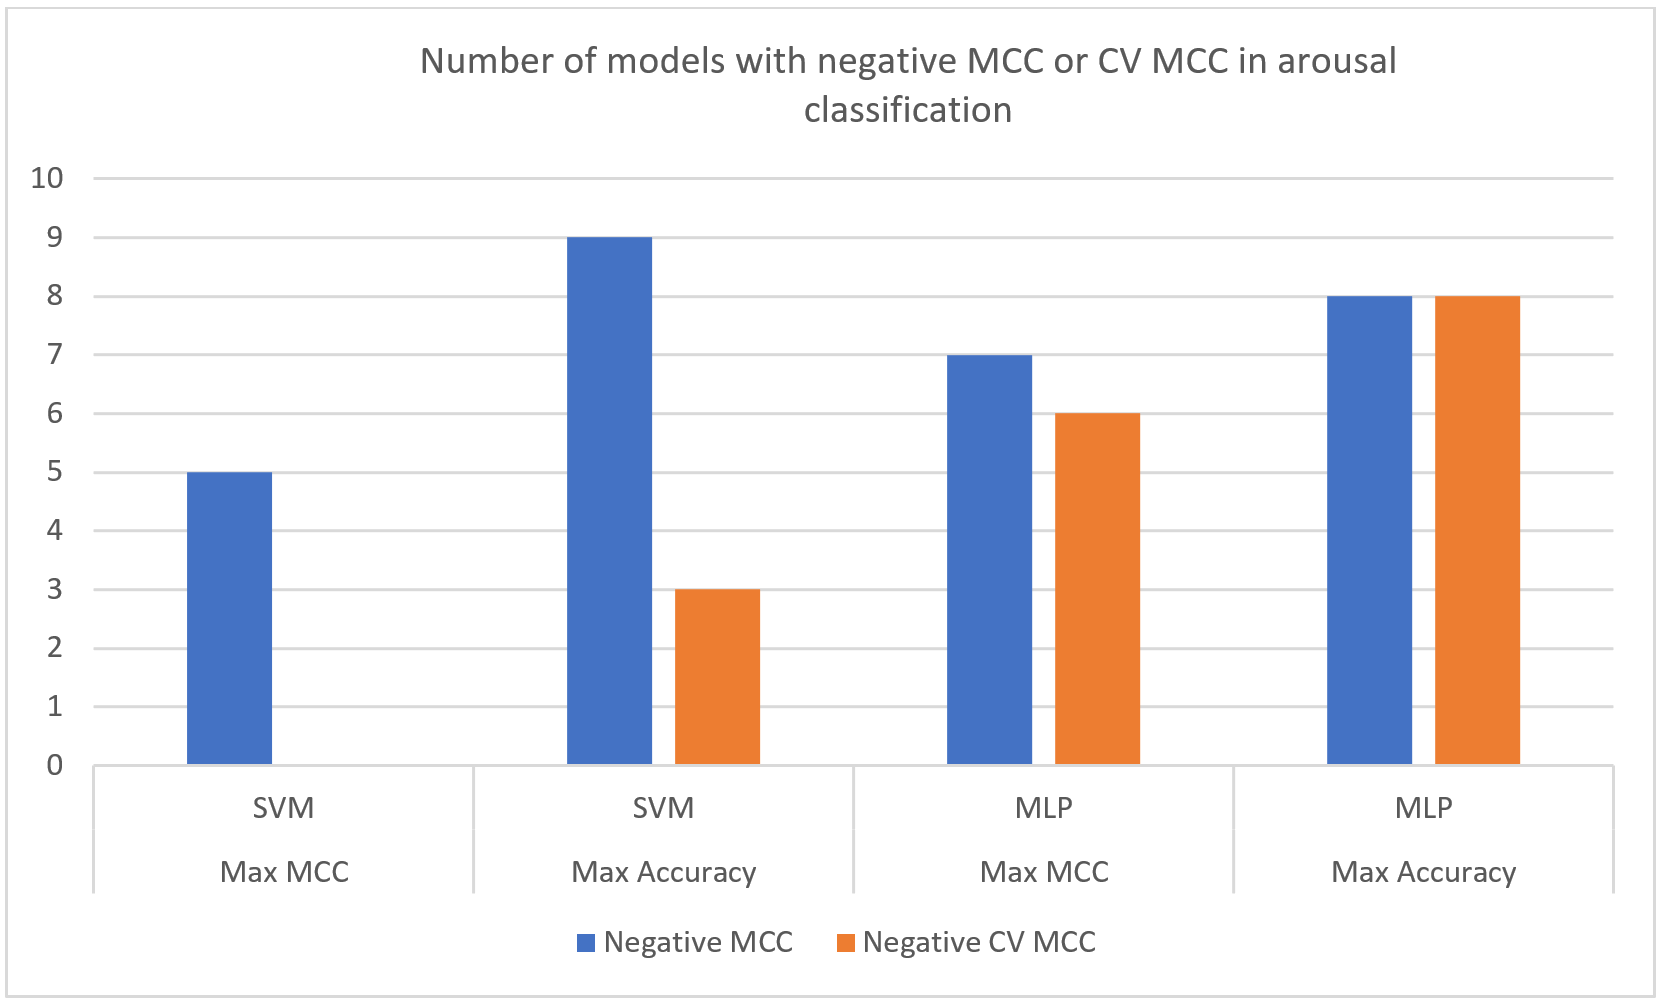
\includegraphics[width=12cm]{img/results/arousal_strategy_comparison.png}
\centering
\caption{Comparison between optimization strategies of negative MCC and CV MCC scores counts for arousal classification.} \label{fig:arousal_strategy_comparison}
\end{figure}

For arousal classification the difference between Max MCC strategy is evident and significant for \ac{SVM} classifiers, and there is increasing trend between Max MCC strategy and Max Accuracy Strategy. In valence classification the difference is less remarkable, but the same increasing trend between the two strategies is present.

\begin{figure}[h!]
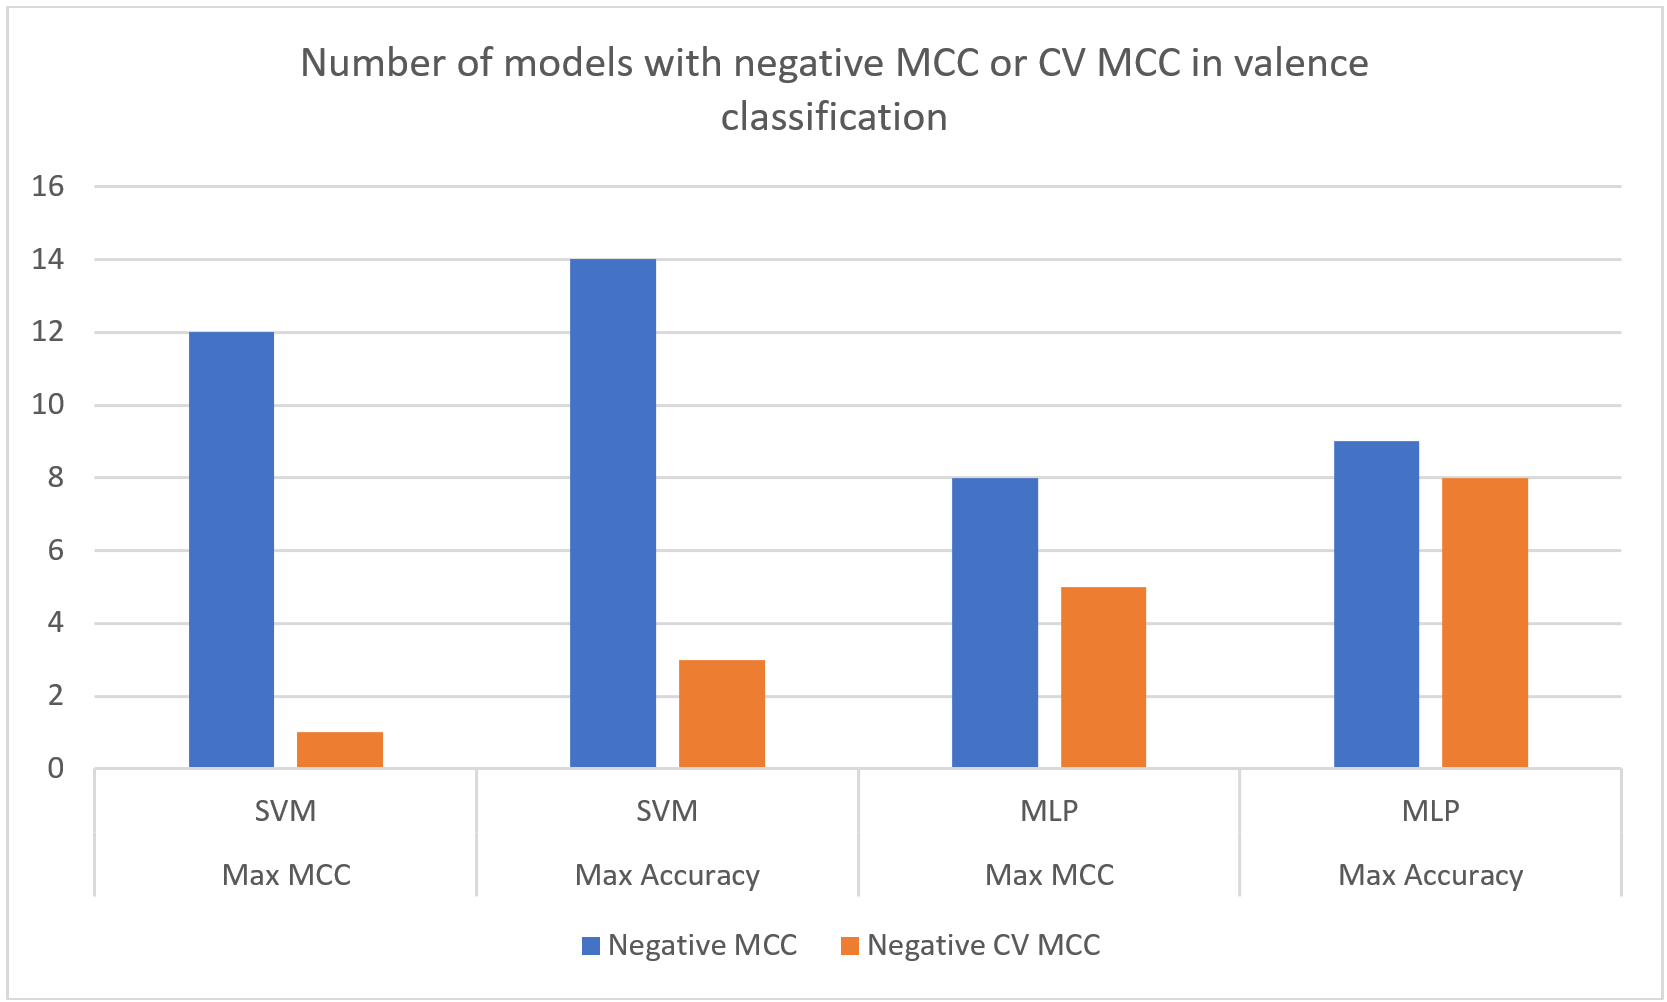
\includegraphics[width=12cm]{img/results/valence_strategy_comparison.png}
\centering
\caption{Comparison between optimization strategies of negative MCC and CV MCC scores counts for arousal classification.} \label{fig:valence_strategy_comparison}
\end{figure}

The current research is more focused on obtaining more interpretable and valid results from the classification of emotional valence and arousal rather than blindly maximizing the accuracy scores of the classifiers. The “Max Accuracy” strategy is less benevolent towards a general approach and generates more over-fitted or under-fitted models than “Max MCC” strategy, therefore results obtained using the latter strategy are considered the final ones and compared with the related work in the following section.
\fi
